\documentclass[a4paper,12pt,french]{book}
\usepackage[margin=2cm]{geometry}
\usepackage[thinfonts]{uglix2}
\usepackage{ulem}
\nouveaustyle

\begin{document}
    \titre{NUM\'ERIQUE ET SCIENCES INFORMATIQUES}{}{}

    \begin{center}
        \Large
        \vspace{6cm}
        \textit{Durée de l'épreuve : 3 heures 30}\\[2em]

        \textit{L'usage de la calculatrice n'est pas autorisé}\\[2em]


        \textit{Le candidat traite au choix 3 exercices parmi les 4 exercices proposés}\\[2em]

        \textit{Chaque exercice devra être traité sur une copie séparée}
    \end{center}
    \newpage

\section*{Exercice 1 \small{\hfill arbres et programmation orientée objet}}

    Une agence immobilière développe un programme pour gérer les biens immobiliers qu’elle propose à la vente.\\
    Dans ce programme, pour modéliser les données de biens immobiliers, on définit une classe \pythoninline{Bim} avec les attributs suivants :
    \begin{enumerate}[--]
        \item 	\pythoninline{nt} de type \pythoninline{str} représente la nature du bien (appartement, maison, bureau, commerces, \textit{et c\ae tera}) ;
        \item	\pythoninline{sf} de type \pythoninline{float} est la surface du bien ;
        \item 	\pythoninline{pm} de type \pythoninline{float} est le prix moyen par m² du bien qui dépend de son emplacement.
    \end{enumerate}

    La classe \pythoninline{Bim} possède une méthode \pythoninline{estim_prix} qui renvoie une estimation du prix du bien.
    Le code (incomplet) de la classe \pythoninline{Bim} est donné ci-dessous :
\begin{pythoncode}
class Bim:
    def __init__(self, nature, surface, prix_moy):
    ...

    def estim_prix(self):
        return self.sf * self.pm
\end{pythoncode}

    \begin{enumerate}[\bfseries 1.]
        \item 	Recopier et compléter le code du constructeur de la classe \pythoninline{Bim}.
        \item 	On exécute l'instruction suivante :\\
                \pythoninline{b1 = Bim('maison', 70.0, 2000.0)}\\
                Que renvoie l'instruction \pythoninline{b1.estim_prix()} ? Préciser le type de la valeur renvoyée.
        \item On souhaite affiner l’estimation du prix d’un bien en prenant en compte sa nature :
        \begin{enumerate}[--]
            \item	pour un bien dont l’attribut \pythoninline{nt} est \pythoninline{'maison'} la nouvelle estimation du prix est le
            produit de sa surface par le prix moyen par m² multiplié par 1,1 ;
            \item 	pour un bien dont l’attribut \pythoninline{nt} est \pythoninline{'bureau'} la nouvelle estimation du prix est le
            produit de sa surface par le prix moyen par m² multiplié par 0,8 ;
            \item pour les autres biens, l'estimation du prix ne change pas.
        \end{enumerate}
        Modifier le code de la méthode \pythoninline{estim_prix} afin de prendre en compte ces changements.
\newpage
        \item Écrire le code Python d'une fonction \pythoninline{nb_maison} qui
        \begin{enumerate}[--]
            \item	prend en argument une liste \pythoninline{lst} d'objets de la classe \pythoninline{Bim} ;
            \item 	renvoie le nombre d’objets de nature \pythoninline{'maison'} contenus dans \pythoninline{lst}.
        \end{enumerate}
        \item  Pour une recherche efficace des biens immobiliers selon le critère de leur surface, on
        stocke les objets de la classe \pythoninline{Bim} dans un arbre binaire de recherche, nommé \pythoninline{abr}.\\
        Pour tout nœud de cet arbre :
        \begin{enumerate}[--]
            \item 	tous les objets de son sous-arbre gauche ont une surface inférieure ou égale à la
            surface de l’objet contenue dans ce nœud ;
            \item 	tous les objets de son sous-arbre droit ont une surface strictement supérieure à la
            surface de l’objet contenue dans ce nœud.
        \end{enumerate}
        \pythoninline{abr} est lui-même un objet et dispose des \textbf{méthodes} suivantes :
        \begin{enumerate}[--]
            \item 	 \pythoninline{abr.est_vide} ne prend aucun paramètre d'entrée, renvoie \pythoninline{True} si \pythoninline{abr} est vide et \pythoninline{False} sinon.
            \item    \pythoninline{abr.get_v} ne prend aucun paramètre d'entrée, renvoie l’élément situé à la racine de \pythoninline{abr} si \pythoninline{abr} n’est pas vide et \pythoninline{None} sinon.
            \item    \pythoninline{abr.get_g} : ne prend aucun paramètre d'entrée, renvoie le sous-arbre gauche de \pythoninline{abr} si \pythoninline{abr} n’est pas vide et \pythoninline{None} sinon.
            \item    \pythoninline{abr.get_f} : ne prend aucun paramètre d'entrée, renvoie le sous-arbre droit de \pythoninline{abr} si \pythoninline{abr} n’est pas vide et \pythoninline{None} sinon.
         \end{enumerate}
         \begin{enumerate}[\bfseries a.]
             \item 	Dans cette question, on suppose que l'arbre binaire \pythoninline{abr} a la forme ci-dessous :
                    \begin{center}
                        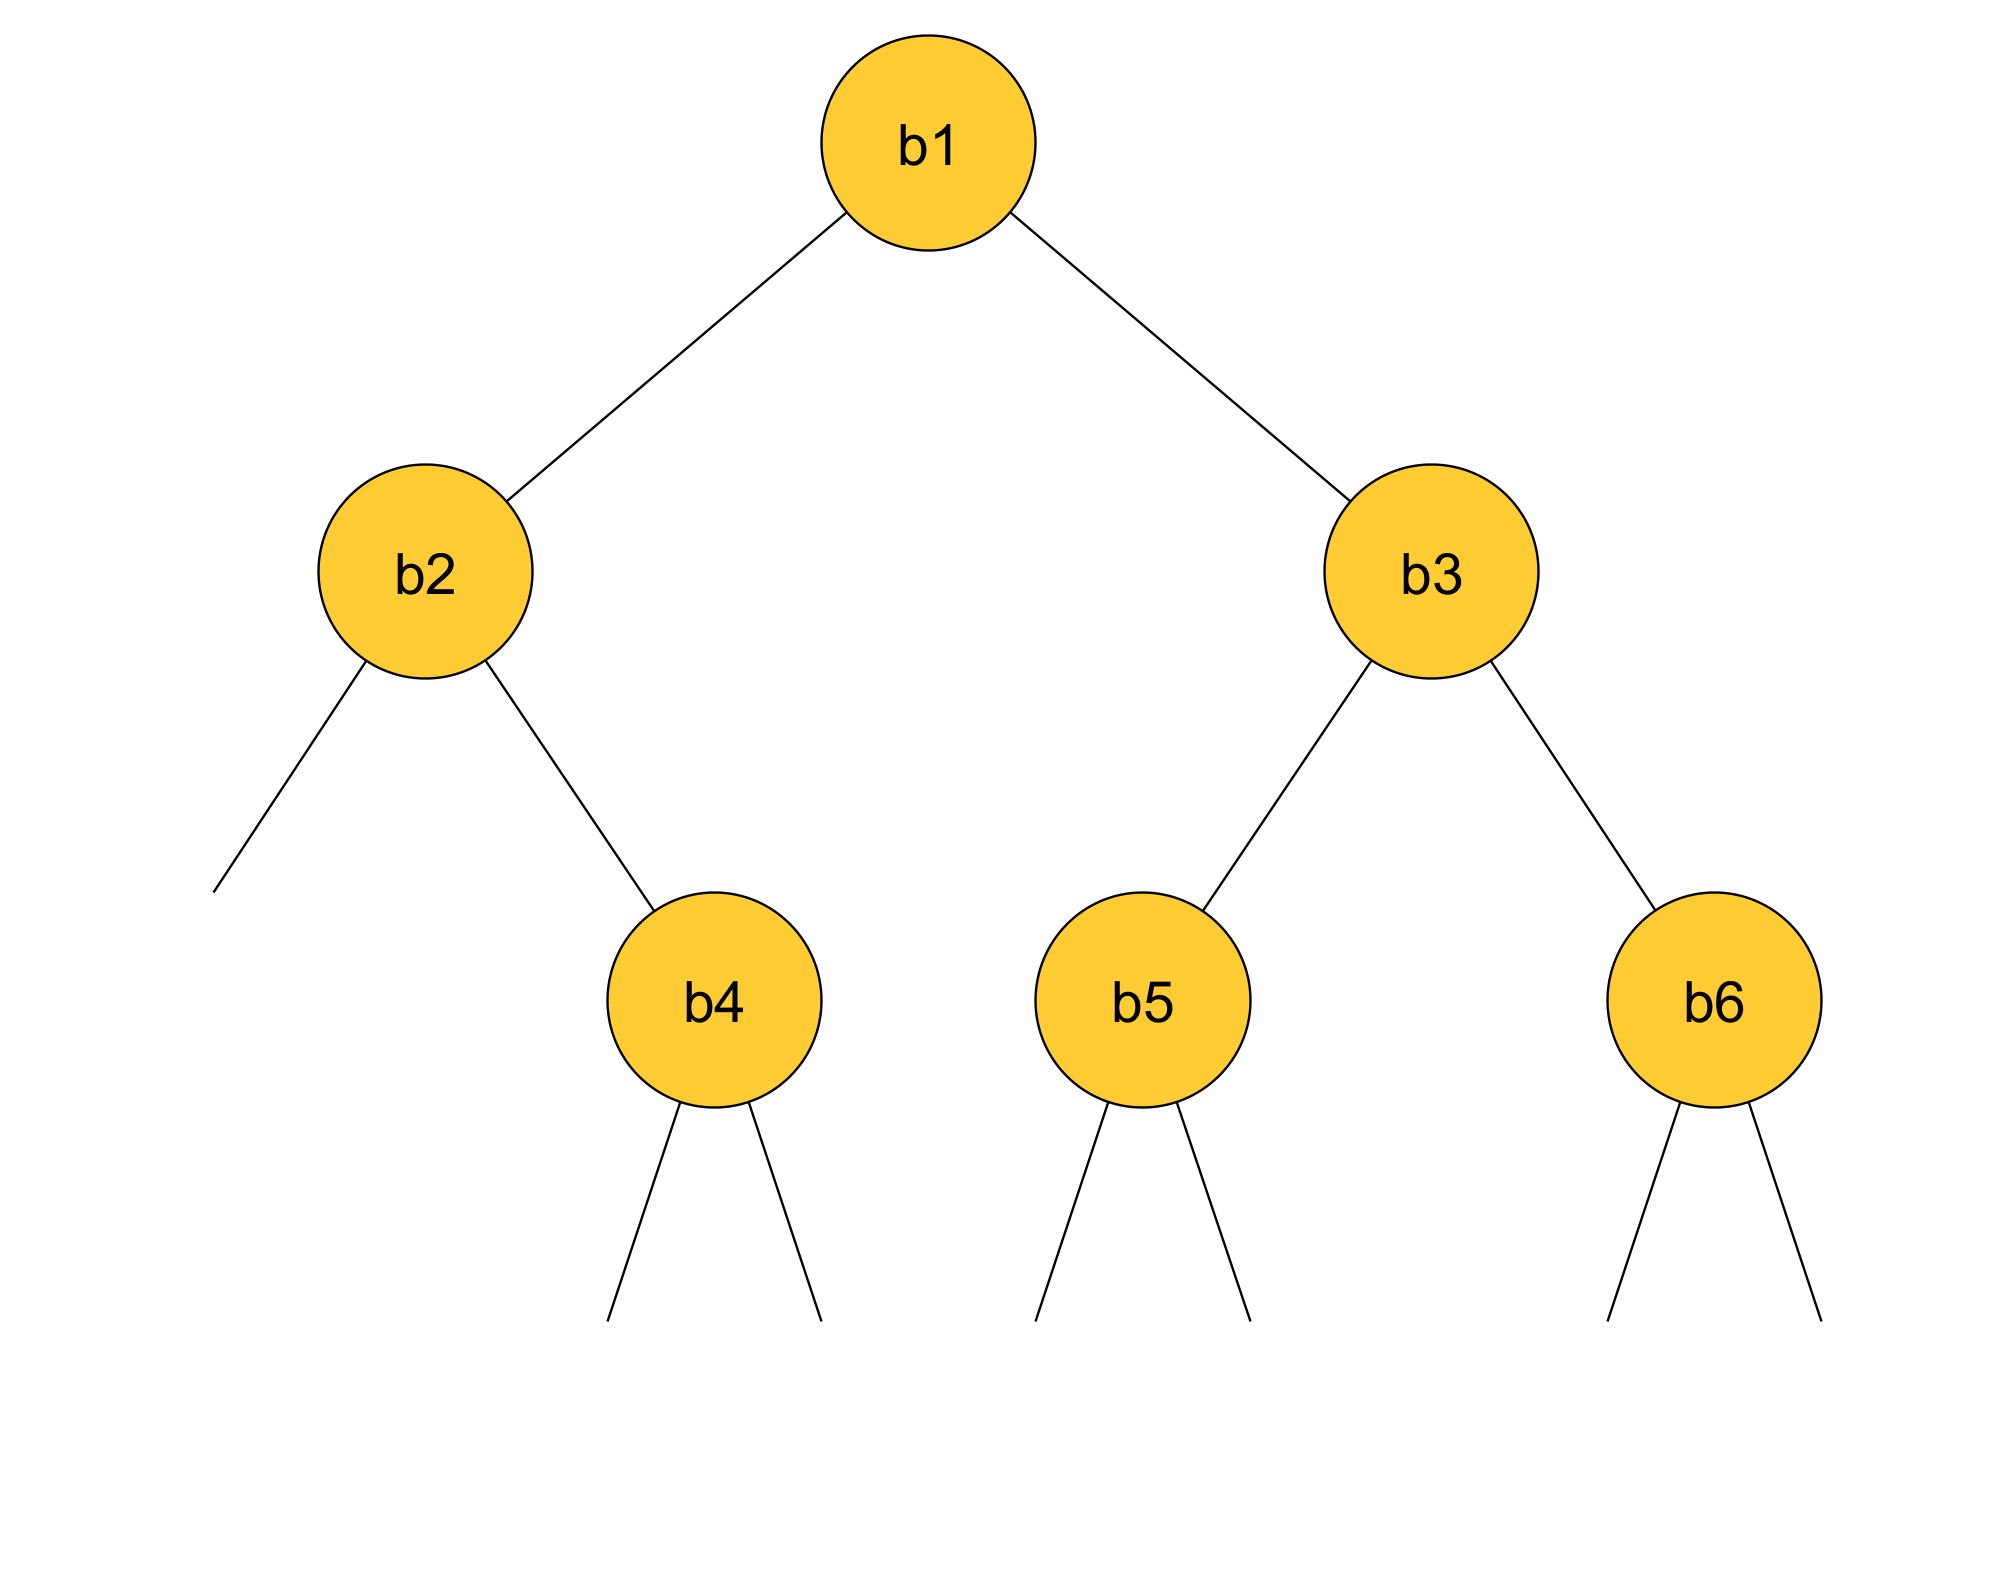
\includegraphics[width=9cm]{img/arbre.png}
                    \end{center}
                    Donner la liste des biens triée dans l'ordre croissant de leur surface en expliquant la méthode choisie.
             \item 	Recopier et compléter le code de la fonction récursive \pythoninline{contient} donnée ci-dessous, qui
             \begin{enumerate}[--]
                 \item 	prend en arguments un nombre \pythoninline{surface} de type \pythoninline{float} et un arbre binaire de recherche \pythoninline{abr} contenant des éléments de la classe \pythoninline{Bim} ordonnés selon leur attribut de surface \pythoninline{sf} ;
                 \item 	renvoie \pythoninline{True} s'il existe un bien dans \pythoninline{abr} d'une
                 surface supérieure ou égale à surface et \pythoninline{False} sinon.
             \end{enumerate}
\begin{pythoncode}
def contient(surface, abr):
    if abr.est_vide():
        return False
    elif abr.get_v().sf >= ......... :
        return True
    else:
        return contient( surface , ......... )
\end{pythoncode}
         \end{enumerate}
    \end{enumerate}


\section*{Exercice 2 \small{\hfill bases de données, langage SQL}}

    L’énoncé de cet exercice utilise les mots du langage SQL suivants :\\

    \mintinline{SQL}{SELECT FROM, WHERE, JOIN ON, INSERT INTO VALUES}\\
    \mintinline{SQL}{UPDATE, SET, DELETE, COUNT, AND, OR}\\

    Pour la gestion des réservations clients, on dispose d’une base de données nommée \texttt{gare} dont le schéma relationnel est le suivant :\\

    \texttt{\textbf{Train} (\uline{numT}, provenance, destination, horaireArrivee, horaireDepart)}\\

    \texttt{\textbf{Reservation} (\uline{numR}, nomClient, prenomClient, prix, \dashuline{numT})}\\

    Les attributs soulignés en trait plein sont des clés primaires. L’attribut souligné en pointillés est une clé étrangère : \texttt{Reservation.numT} fait référence à la clé primaire \texttt{Train.numT}.\\

    Les attributs \texttt{horaireDepart} et \texttt{horaireArrivee} sont de type \mintinline{SQL}{TIME} et s’écrivent selon le format \texttt{hh:mm}, où \texttt{hh} représente les heures et \texttt{mm} les minutes.\\

    \begin{enumerate}[\bfseries 1.]
        \item Quel nom générique donne-t-on aux logiciels qui assurent, entre autres, la persistance des données, l’efficacité de traitement des requêtes et la sécurisation des accès pour les bases de données ?
        \item \begin{enumerate}[\bfseries a.]
            \item On considère les requêtes SQL suivantes :

\begin{sql}
DELETE FROM Train WHERE numT = 1241 ;
DELETE FROM Reservation WHERE numT = 1241 ;
\end{sql}

            Sachant que le train n°1241 a été enregistré dans la table \texttt{Train} et que des réservations pour ce train ont été enregistrées dans la table \texttt{Reservation}, expliquer pourquoi cette suite d’instructions renvoie une erreur.
            \item Citer un cas pour lequel l’insertion d’un enregistrement dans la table \texttt{Reservation} n’est pas possible.

        \end{enumerate}
        \item Écrire des requêtes SQL correspondant à chacune des instructions suivantes :
        \begin{enumerate}[\bfseries a.]

            \item Donner tous les numéros des trains dont la destination est « Lyon ».
            \item Ajouter une réservation n°1307 de 33 € pour M. Alan Turing dans le train n°654.
            \item Suite à un changement, l’horaire d’arrivée du train n°7869 est programmé à 08: 11.\\
            Mettre à jour la base de données en conséquence.
            \item Produire la table des noms et prénoms de tous les clients qui ont effectué une réservation pour un train partant de Paris et allant à Marseille.
        \end{enumerate}
    \end{enumerate}



\section*{Exercice 3 \small{\hfill structures de données linéaires}}

    Une méthode simple pour gérer l'ordonnancement des processus est d'exécuter les processus en une seule fois et dans leur ordre d'arrivée.\\

    \begin{enumerate}[\bfseries 1.]
        \item Parmi les propositions suivantes, quelle est la structure de données la plus appropriée pour mettre en œuvre le mode FIFO (First In First Out) ?
        \begin{enumerate}[\bfseries a.]
            \item liste
            \item dictionnaire
            \item pile
            \item file
        \end{enumerate}
        \item On choisit de stocker les données des processus en attente à l'aide d'une liste Python \pythoninline{lst}. On dispose déjà d'une fonction \pythoninline{retirer(lst)} qui renvoie l'élément \pythoninline{lst[0]} puis le supprime de la liste \pythoninline{lst}.\\

        Écrire en Python le code d'une fonction \pythoninline{ajouter(lst, proc)} qui ajoute à la fin de la liste \pythoninline{lst} le nouveau processus en attente \pythoninline{proc}.

        \item On choisit maintenant d'implémenter une file \pythoninline{file} à l'aide d'un couple \pythoninline{(p1,p2)} où \pythoninline{p1} et \pythoninline{p2} sont des piles. Ainsi \pythoninline{file[0]} et \pythoninline{file[1]} sont respectivement les piles \pythoninline{p1} et \pythoninline{p2}.
        \begin{enumerate}[--]
            \item Pour enfiler un nouvel élément \pythoninline{elt} dans file, on l'empile dans \pythoninline{p1}.
            \item Pour défiler file, deux cas se présentent :
            \begin{enumerate}[\textbullet]
                \item La pile \pythoninline{p2} n'est pas vide : on dépile \pythoninline{p2}.
                \item La pile \pythoninline{p2} est vide : on dépile les éléments de \pythoninline{p1} en les empilant dans \pythoninline{p2} jusqu'à ce que \pythoninline{p1} soit vide, puis on dépile \pythoninline{p2}.
            \end{enumerate}
        \end{enumerate}
        \begin{center}
            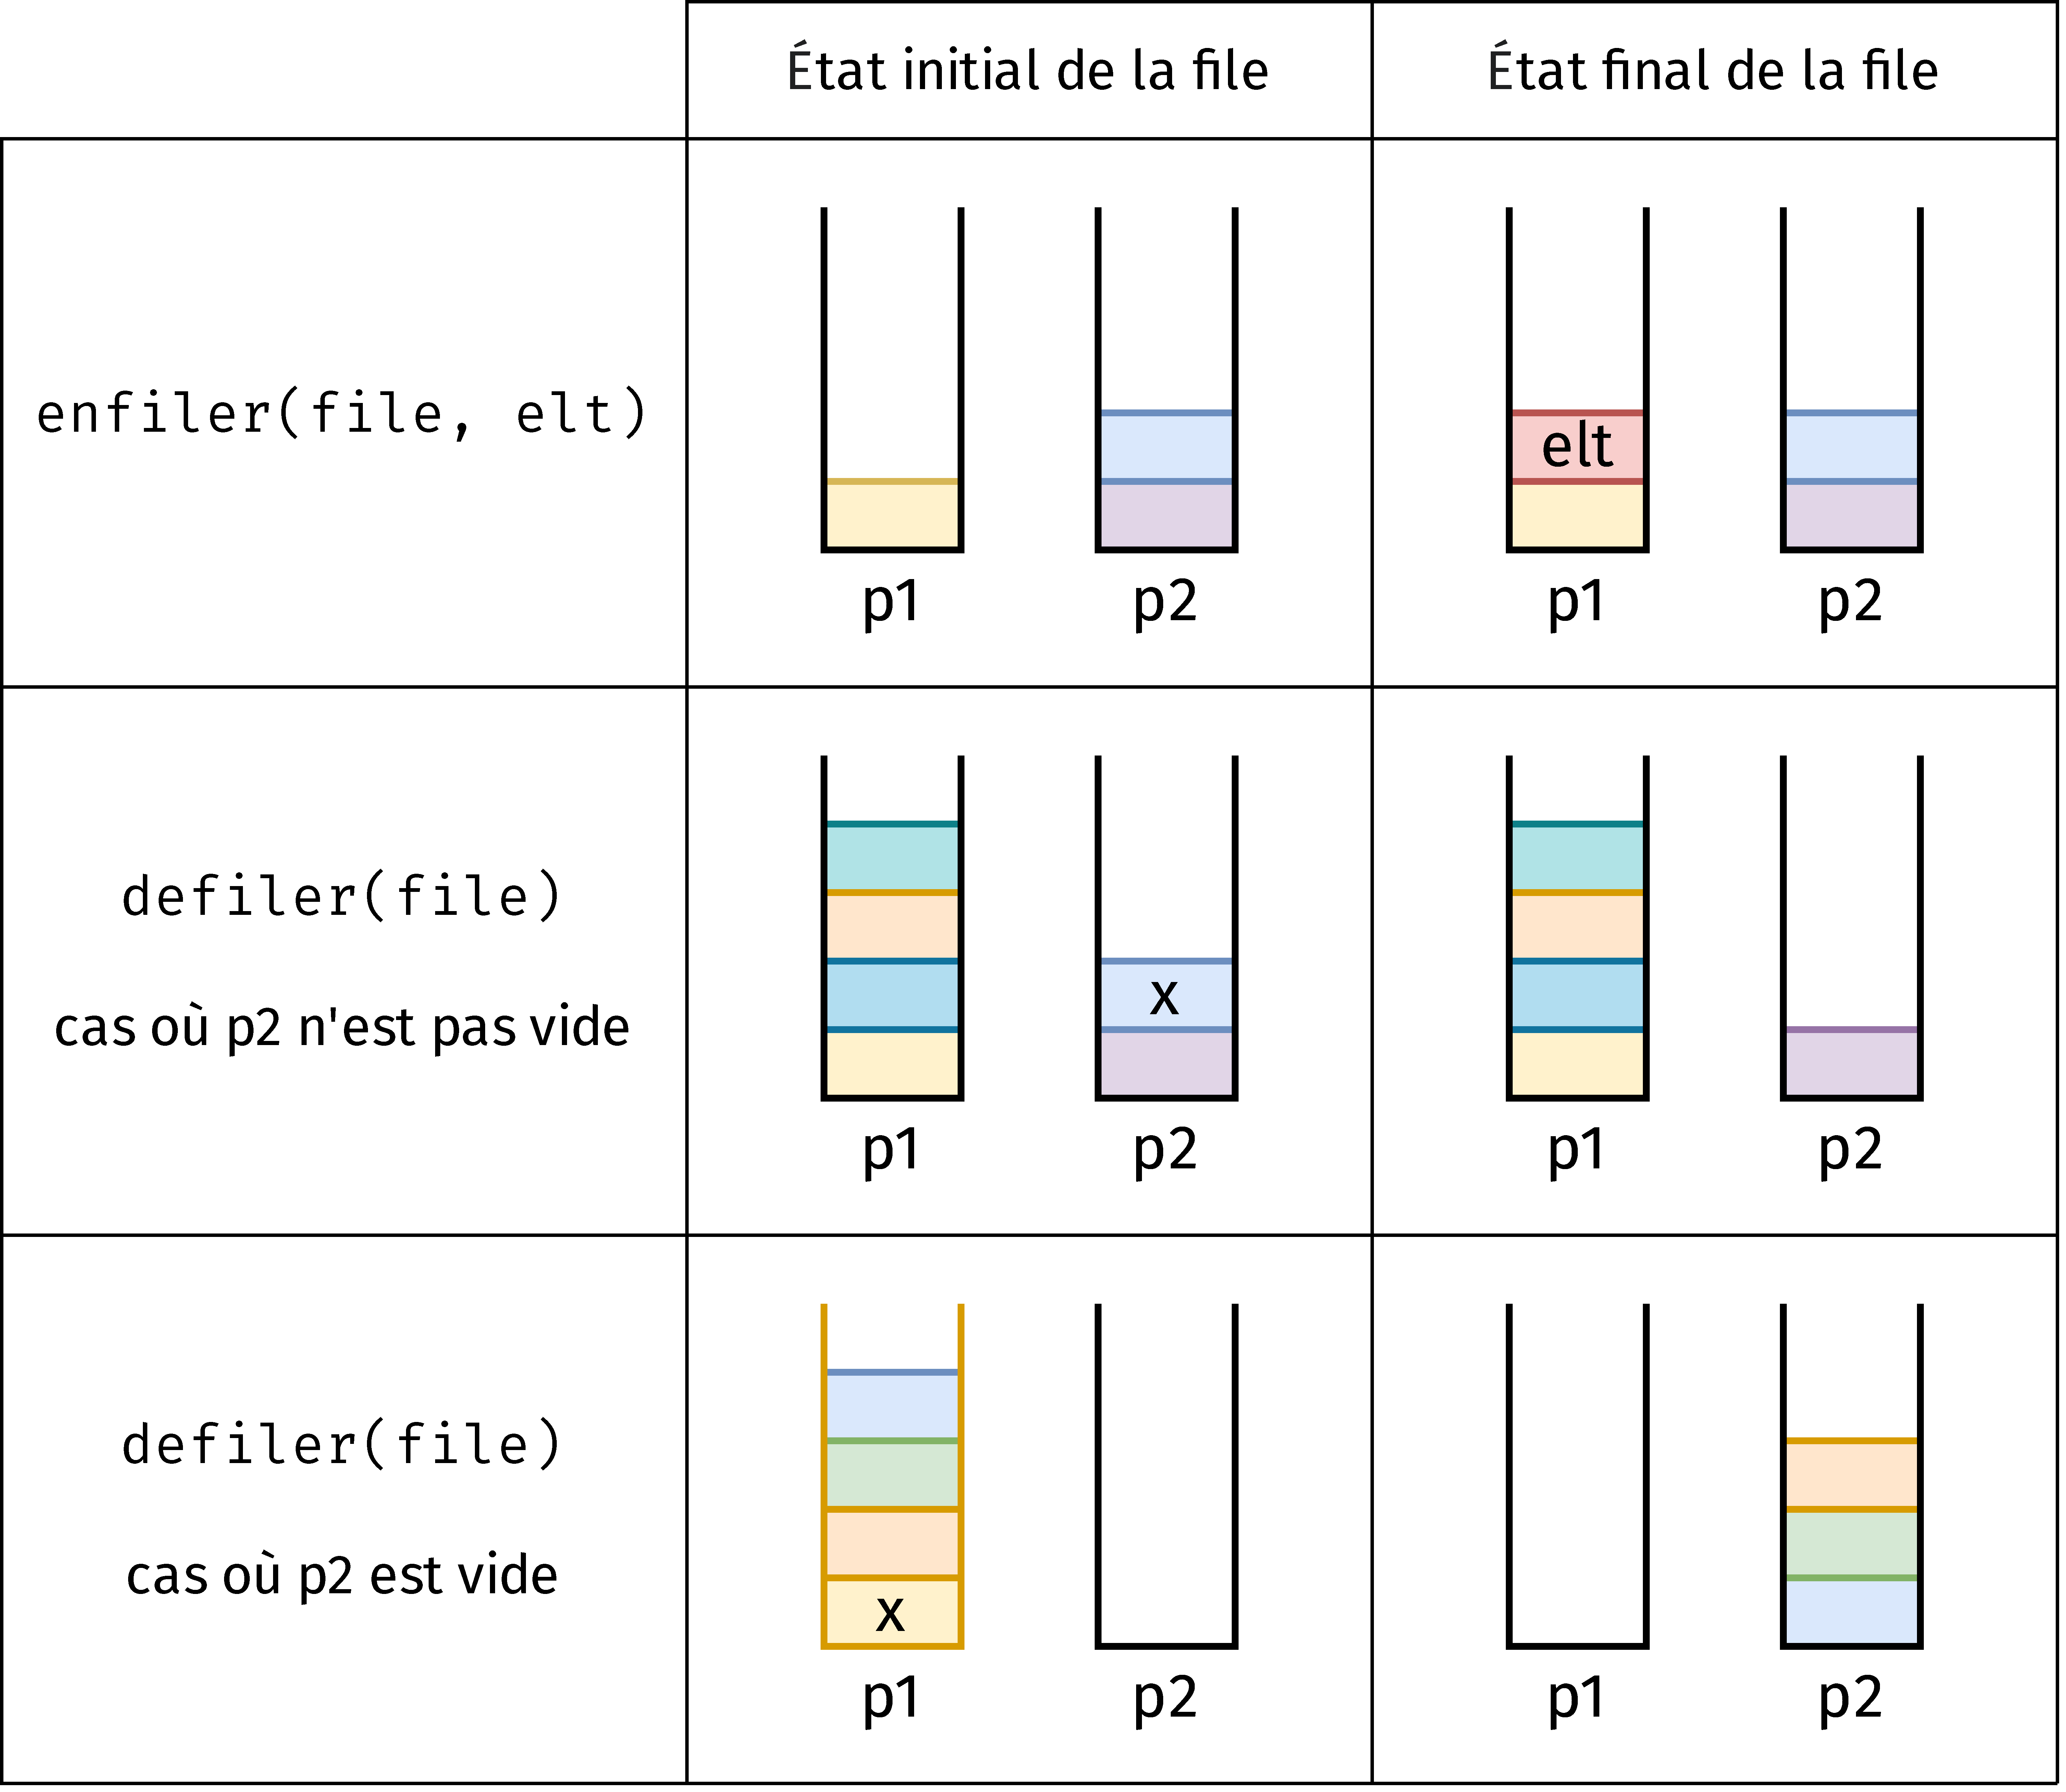
\includegraphics[width=10cm]{img/file2piles}
        \end{center}
        On considère la situation représentée ci-dessous.
        \begin{center}
            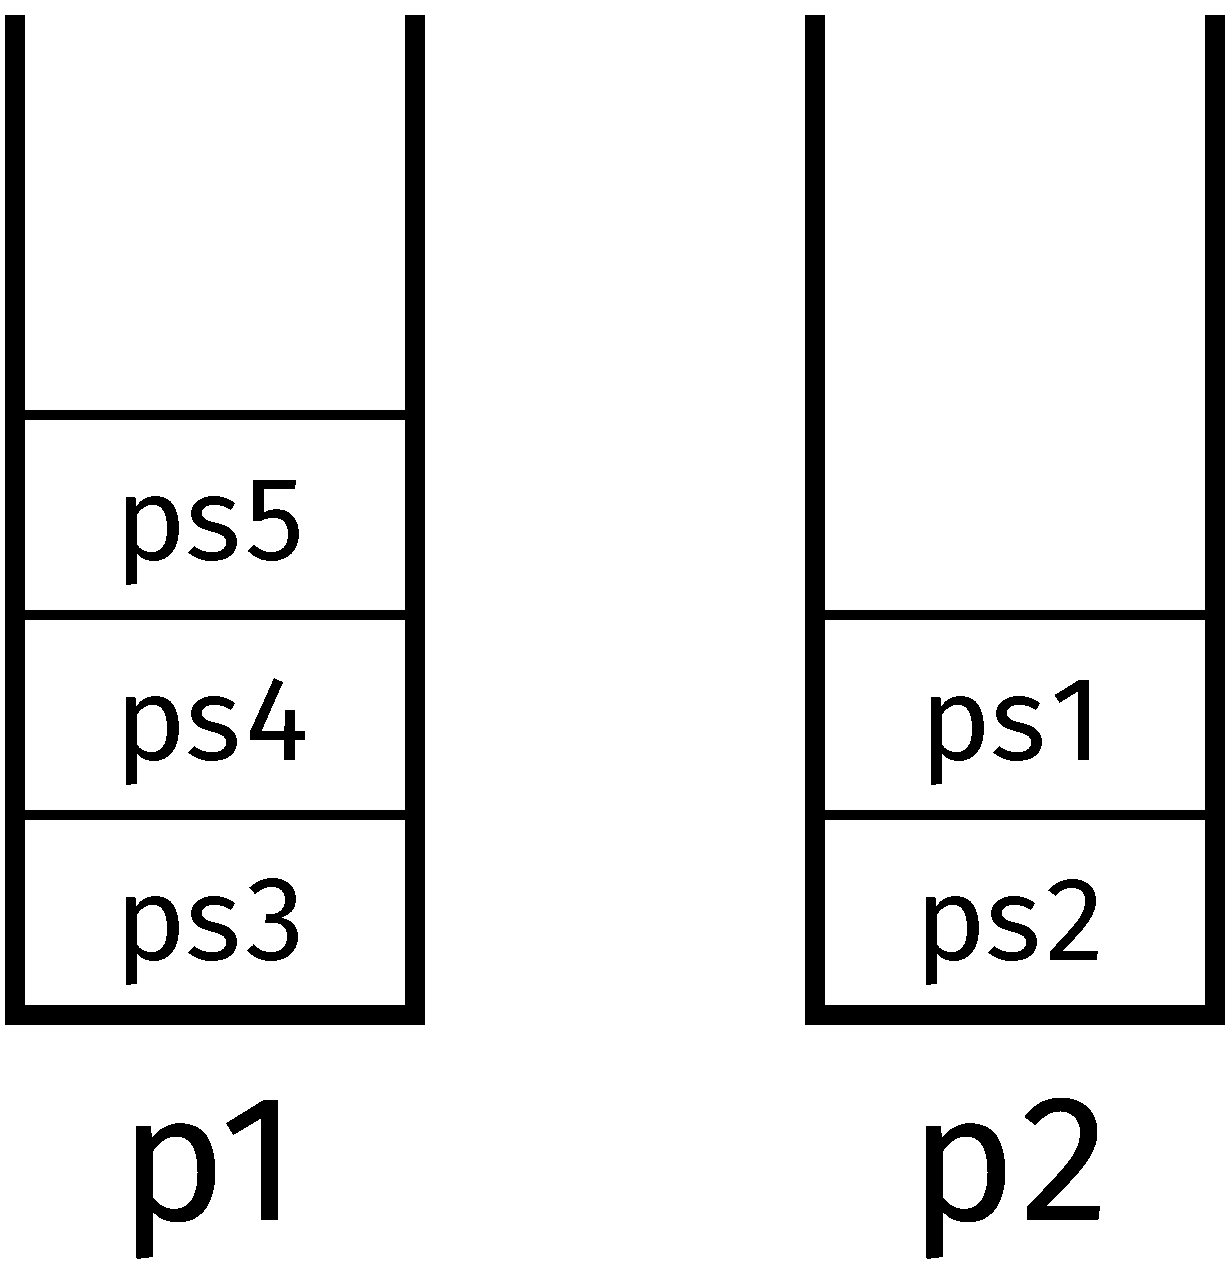
\includegraphics[width=2.1cm]{img/file2piles2}
        \end{center}
        On exécute la séquence d'instructions suivante :
\begin{minted}{python}
enfiler(file, ps6)
defiler(file)
defiler(file)
defiler(file)
enfiler(file, ps7)
\end{minted}
        Représenter le contenu final des deux piles à la suite de ces instructions.


        \item
        On dispose des fonctions :
        \begin{enumerate}[--]
            \item \pythoninline{empiler(p,elt)} qui empile l'élément \pythoninline{elt} dans la pile \pythoninline{p};
            \item \pythoninline{depiler(p)} qui renvoie le sommet de la pile \pythoninline{p} si \pythoninline{p} n'est pas vide et le supprime;
            \item \pythoninline{pile_vide(p)} qui renvoie \pythoninline{True} si la pile \pythoninline{p} est vide, \pythoninline{False} si la pile \pythoninline{p} n'est pas vide.
        \end{enumerate}

        \begin{enumerate}[\bfseries a.]
            \item Écrire en Python une fonction \pythoninline{est_vide(f)} qui prend en argument un \textit{couple de piles} \pythoninline{f} et qui renvoie \pythoninline{True} si la file représentée par \pythoninline{f} est vide, \pythoninline{False} sinon.
            \item  Écrire en Python une fonction \pythoninline{enfiler(f,elt)} qui prend en arguments un \textbf{couple de piles} \pythoninline{f} et un élément \pythoninline{elt} et qui ajoute \pythoninline{elt} en queue de la file représentée par \pythoninline{f}.
            \item Écrire en Python une fonction \pythoninline{defiler(f)} qui prend en argument un \textbf{couple de piles} \pythoninline{f} et qui renvoie l'élément en tête de la file représentée par \pythoninline{f} en le retirant. On supposera que la file \texttt{f} n'est pas vide.
        \end{enumerate}
    \end{enumerate}

\section*{Exercice 4 \small{\hfill gestion des processus et ressources}}

    Les parties A et B peuvent être traitées indépendamment.

    \subsection*{Partie A}

    Dans un bureau d’architectes, on dispose de certaines ressources qui ne peuvent être utilisées simultanément par plus d’un processus, comme l’imprimante, la table traçante, le modem.\\
    Chaque programme, lorsqu'il s’exécute, demande l'allocation des ressources qui lui sont nécessaires. Lorsqu'il a fini de s’exécuter, il libère ses ressources.
     \begin{center}
        \begin{tabular}{|c|c|c|}
            \hline
            \rowcolor{UGLiOrange} \textbf{\color{white}Programme 1 }& \textbf{\color{white}Programme 2} & \textbf{\color{white}Programme 3}  \\
            \hline
            demander table traçante & demander modem & demander imprimante \\
            \hline
            demander modem& demander imprimante & demander table traçante  \\
            \hline
            exécution& exécution & exécution   \\
            \hline
            libérer modem& libérer imprimante & libérer table traçante   \\
            \hline
            libérer table traçante& libérer modem & libérer imprimante   \\
            \hline
        \end{tabular}
    \end{center}
    On appelle P1, P2 et P3 les processus respectivement associés aux programmes 1, 2 et 3. Ces processus s'effectuent de manière concurrente.

    \begin{enumerate}[\bfseries 1.]
        \item 	Justifier qu'une situation d'interblocage peut se produire.
        \item 	Modifier l'ordre des instructions du programme 3 pour qu'une telle situation ne puisse pas se produire (aucune justification n'est attendue).
        \item 	Supposons que le processus P1 demande la table traçante alors qu'elle est en cours d'utilisation par le processus P3.\\
                Parmi les états suivants, quel sera l'état du processus P1 tant que la table traçante n'est pas disponible ?

                \begin{multicols}{4}
                    \begin{enumerate}[\bfseries a.]
                        \item 	élu
                        \item 	bloqué
                        \item 	prêt
                        \item 	terminé
                    \end{enumerate}
                \end{multicols}
    \end{enumerate}

    \subsection*{Partie B}
    Avec une ligne de commande dans un terminal sous Linux, on obtient l'affichage suivant :
    \begin{center}
        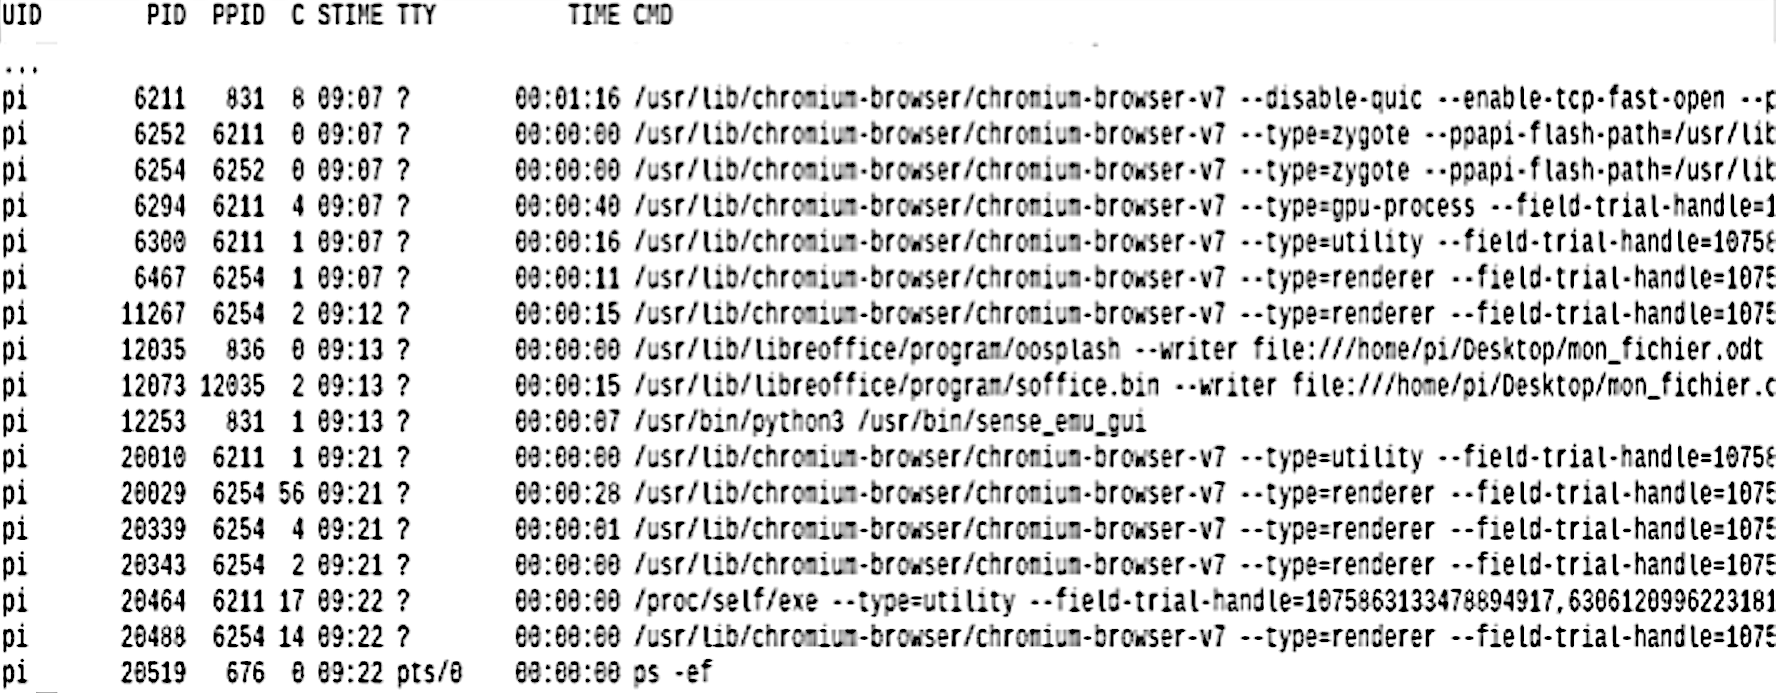
\includegraphics[width=\linewidth]{img/ps}
    \end{center}

    La documentation Linux donne la signification des différents champs :
    \begin{enumerate}[--]
        \item 	UID : identifiant utilisateur effectif ;
        \item	PID : identifiant de processus ;
        \item	PPID : PID du processus parent ;
        \item	C : partie entière du pourcentage d'utilisation du processeur par rapport au temps de vie des processus ;
        \item	STIME : l'heure de lancement du processus ;
        \item	TTY : terminal de contrôle ;
        \item	TIME : temps d'exécution ;
        \item	CMD :  nom de la commande du processus.
    \end{enumerate}
    \begin{enumerate}[\bfseries 1.]
        \item  Parmi les quatre commandes suivantes, laquelle a permis cet affichage ?
                \begin{multicols}{2}
                    \begin{enumerate}[\bfseries a.]
                        \item \texttt{ls -l}
                        \item \tw{ps –ef}
                        \columnbreak
                        \item \tw{cd ..}
                        \item \tw{chmod 741 processus.txt}
                    \end{enumerate}
                \end{multicols}
  	     \item Quel est l'identifiant du processus parent à l'origine de toues les processus concernant le navigateur Web (chromium-browser) ?
         \item Quel est l'identifiant du processus dont le temps d'exécution est le plus long ?
    \end{enumerate}
\end{document}